\documentclass[	11pt, ]{fphw}

\usepackage[utf8]{inputenc} 
\usepackage[T1]{fontenc}
\usepackage{mathpazo}\usepackage{graphicx} 
\usepackage{booktabs} 
\usepackage{listings} 
\usepackage{amsmath}
\usepackage{eso-pic}
\usepackage{array}
\usepackage{float}
\usepackage{graphicx}
\usepackage{bbm}
\usepackage{transparent}
\usepackage{indentfirst}
\usepackage{amsthm}
\usepackage{amsmath,amssymb}
\usepackage{subfigure}
\usepackage{tabu}
\usepackage{enumitem}
\usepackage{caption,tabularx,booktabs}
\usepackage{enumerate} 
\usepackage[english]{varioref}

\renewcommand{\thesection}{\Roman{section}}
\usepackage{titlesec}
\titleformat{\section}
{\normalfont\Large\bfseries}{Exercise~\thesection}{1em}{}
\makeatletter
\renewcommand{\@seccntformat}[1]{%
  \csname the#1\endcsname
  \csname suffix@#1\endcsname % this does nothing unless \suffix@... is defined
  \quad
}
% the subsection number is just a letter
\renewcommand{\thesubsection}{\alph{subsection}}
% but references will also have “section.subsection.” in front of the letter
\renewcommand{\p@subsection}{\thesubsection.}
% define \suffix@subsection
\newcommand{\suffix@subsection}{)}
\makeatother

\title{Assignment \#5} %
\author{Anita Mezzetti} 
\institute{École polytechnique fédérale de Lausanne} 
\class{Global Business Environment} 
\professor{Luisa Lambertini} 

%--------------------------------------------------------------------
\begin{document}
\maketitle 
\section{}
\subsection{}

The Taylor rule states that:
\begin{align}
    r_{t} = & real^{*}+ \pi _{t} + \phi_{\pi} (\pi _{t}- \pi^{*}) + \phi_{y} * 100 * (\frac{y_{t}-\overline{y}_{t}}{\overline{y}_{t}}) = \\
    = & 2 + \pi _{t} + 0.5 ( \pi _{t}- 2) + 50 *  (\frac{y_{t}-\overline{y}_{t}}{\overline{y}_{t}})
\end{align}
\begin{figure}[h] 
\centering 
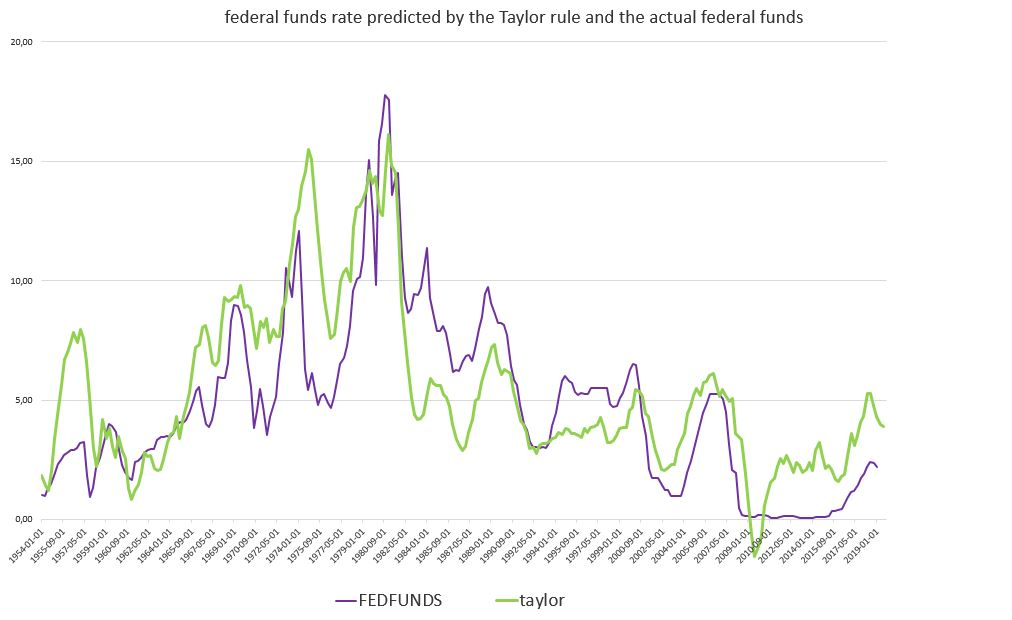
\includegraphics[scale=0.7]{es5a.JPG} 
\caption{Question 1.a} 
\label{11}
\end{figure}




\subsection{}
\begin{figure}[h] 
\centering 
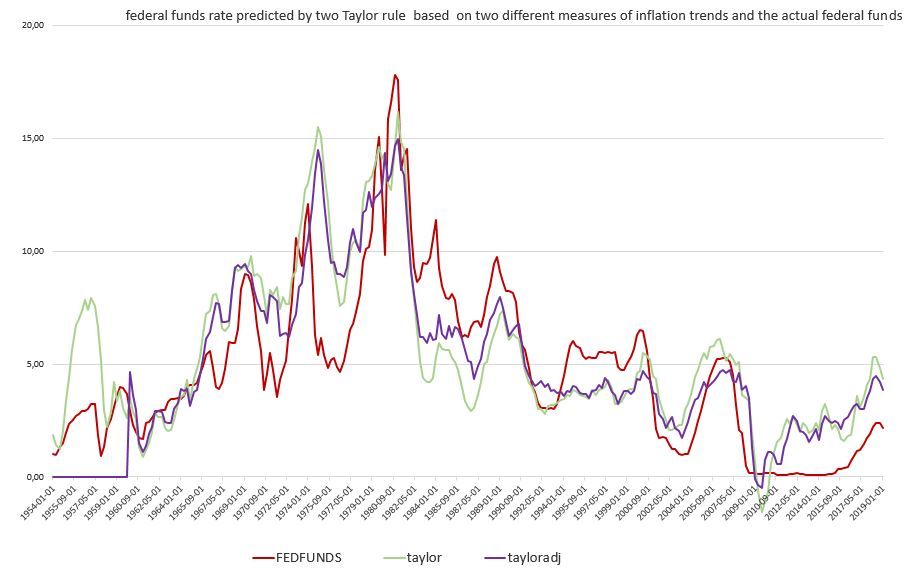
\includegraphics[scale=0.7]{es5b.JPG} 
\caption{Question 1.b} 
\label{11}
\end{figure}
We can see that the differences are smaller using the core inflation. Using it, the situation is more stable than that measured by the implicit GDP deflator. In fact, it does not consider some volatile components, as energy and food. \\
Temporary shocks that raise the prices of food and energy relative to other prices can have considerable effects on the previous inflation rate, which is given by the implicit GDP deflator in the short run. Core inflation is influenced less and it has smaller movements. Therefore, it is better to use this index to do our analysis. \\

However, to explain all the reasons of the difference between the effective and the calculated federal fund rate, we cannot limit our examination to the components of food and energy. 
We should think about the 2001 recession, which leads the FED to low interest rates very sharply (more than the predictions) from 2003 to 2006. While, regarding 2010 gap, we can see that the Effective Federal Funds Rate is lower than the predicted: it has a value of almost zero.  The Fed needed to decrease the rate, but it could not reduce it any further. 

\newpage
\section{}
\subsection{}
We remember the formula
\begin{equation} \label{a}
\frac{M_{0}}{P_{0}}=L(R,Y^{f})
\end{equation}
So, for the home case we have
\begin{align}
    \frac{M_{0}}{P_{0}}= &1,05* Y^{f}-100*R \\
    \frac{100}{1}=&1,05* 100-100*R \\
    R=& -\frac{100-1,05*100}{100}=0,05
\end{align}  

\subsection{}
We use the same formula \ref{a} for the foreign market and we obtain
\begin{align}
    \frac{M^{*}_{0}}{P^{*}_{0}}= &1,6* Y^{*f}-200*R^{*} \\
    \frac{15}{0,1}=&1,6 * 100-200*R^{*} \\
    R^{*}=& -\frac{150-1,6*100}{200}=0,05
\end{align}  


\subsection{}
The real exchange rate states that:
\begin{align}
    q= &\frac{E*P}{P^{*}} \\
    E=E^{e}=E_{0}=&\frac{q*P}{P^{*}}= \\
    =&\frac{1*1}{0,1}=10
\end{align}



\subsection{}
Permanent increase of foreign money supply of 5\% means that money supply moves from $M^{*0}_{s}=15$ to $M^{*1}_{s}=15,75$. 
We calculate the new expected long-run return ex. rate:
\begin{align}
    E^{lr}=&q*\frac{P_{0}}{P^{*}_{1}}=q*\frac{P_{0}* L^{*}}{M^{*1}_{s}} = \\
    =&1*\frac{1*(1,6*100-200*0,05)}{15,75}=9,52
\end{align}
Then, considering $E^{e}=E^{lr}$, we can calculate the E:
\begin{align}
    E=\frac{E^{e}}{R-R^{*}+1}=E^{e}=9,524
\end{align}

\subsection{}
The only thing that changes is the expected exchange rate, which appreciated due to the change in foreign money supply. Home monetary policy is not affected in the short term.  See figure \vref{5e}.
\begin{figure}[h] 
\centering 
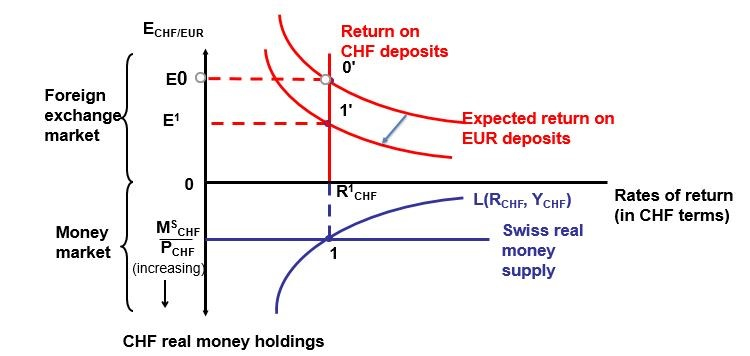
\includegraphics[scale=0.6]{5e.JPG} 
\caption{Question 2.e} 
\label{5e}
\end{figure}

\subsection{}
Foreign money supply is raised to $M^{*1}_{s}=15,75$. So, applying the formula \ref{a} to the foreign market we obtain:
\begin{align}
    \frac{M^{*}_{1}}{P_{0}}= &1,6* Y^{*f}-200*R^{*} \\
    \frac{15,75}{0,1}= &1,6* 100-200*R^{*} \\
    R^{*}=& -\frac{157,5-1,6*100}{200}=0,0125
\end{align}
Then we can calculate the E:
\begin{align}
    E=\frac{E^{e}}{R-R^{*}+1}=\frac{9,524}{0,05-0,0125+1}=9,180
\end{align}

\subsection{}  %g
See figure \vref{5g}.
\begin{figure}[h!] 
\centering 
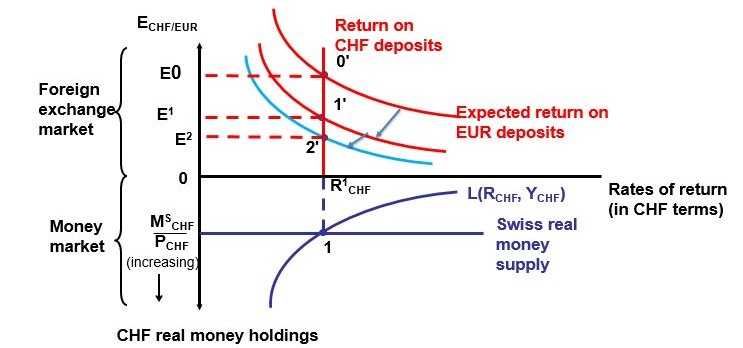
\includegraphics[scale=0.7]{5f.JPG} 
\caption{Question 2.g} 
\label{5g}
\end{figure}

\subsection{}
We do not see any changes in the Home part. See figure \vref{5h}.
\begin{figure}[h!] 
\centering 
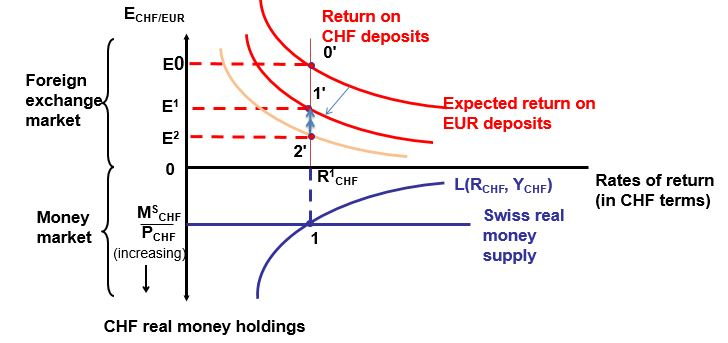
\includegraphics[scale=0.7]{5h.JPG} 
\caption{Question 2.h} 
\label{5h}
\end{figure}

\subsection{}
Permanent increase of home money supply of 5\% means that money supply moves from $M^{0}_{s}=100$ to $M^{1}_{s}=105$. 
We calculate the new expected long-run return ex. rate:
\begin{align}
    E^{lr}=&q*\frac{P_{0}}{P^{*}_{1}}=q*\frac{M^{1}_{s}* L^{*}}{M^{*1}_{s}*L} = \\
    =&1*\frac{105*(1,6*100-200*0,05)}{15,75*(1,05*100-100*0,05)}=10
\end{align}
Then, considering equation \ref{a}:
\begin{align}
\frac{105}{1}=&1,05*100-100*R^{3}\\
R^{3}=&\frac{105-105}{100}=0
\end{align}

Then, considering $E^{e}=E^{lr}$, we can calculate the $E^{3}$:
\begin{align}
    E^{3}=&\frac{E^{e}}{R-R^{*}+1}= \\
   =&\frac{10}{0-0,0125+1}=10,127
\end{align}

\subsection{}
In this figure $R^{3}_{CHF}$ should be zero. However this choice would make the situation a little confusing (due to the presence of the y axis). So we put $R^{3}$ a little right to make it more readable. In this case, the new $E^{3}$ is different from $E^{0}$ because we have a new $R^{3}=0$. See figure \vref{5j}.
\begin{figure}[h] 
\centering 
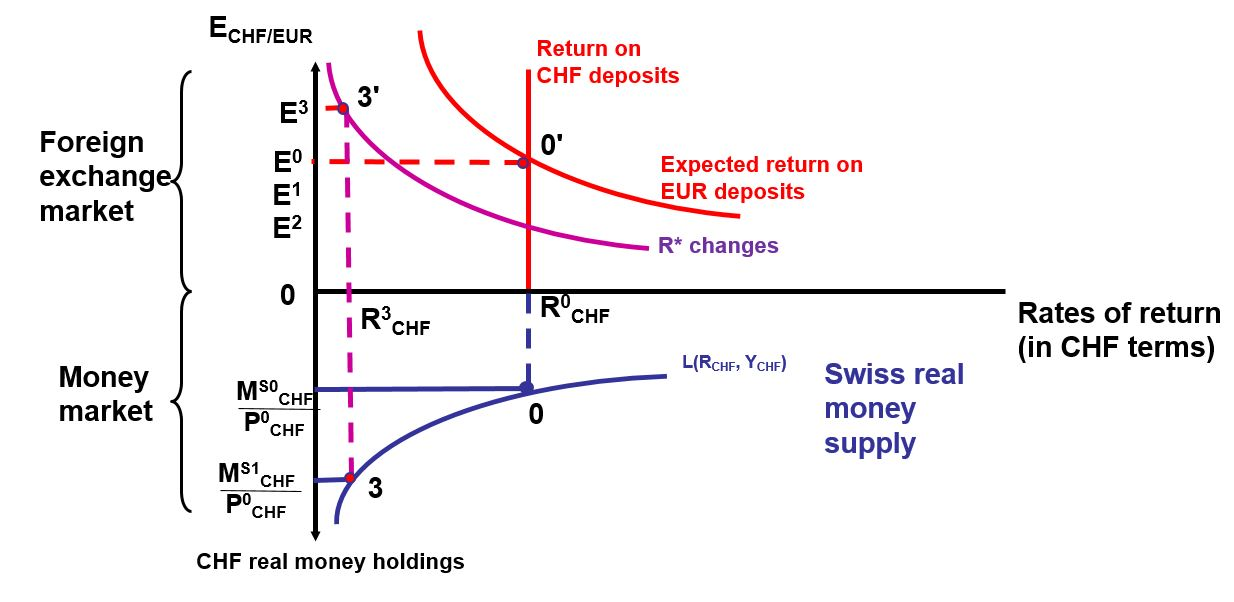
\includegraphics[scale=0.65]{5j.JPG} 
\caption{Question 2.j} 
\label{5j}
\end{figure}

\subsection{}
See figure \vref{5k}. In the long run the home price rises and, consequently, also the interest rate. The same happens abroad.
\begin{figure}[h] 
\centering 
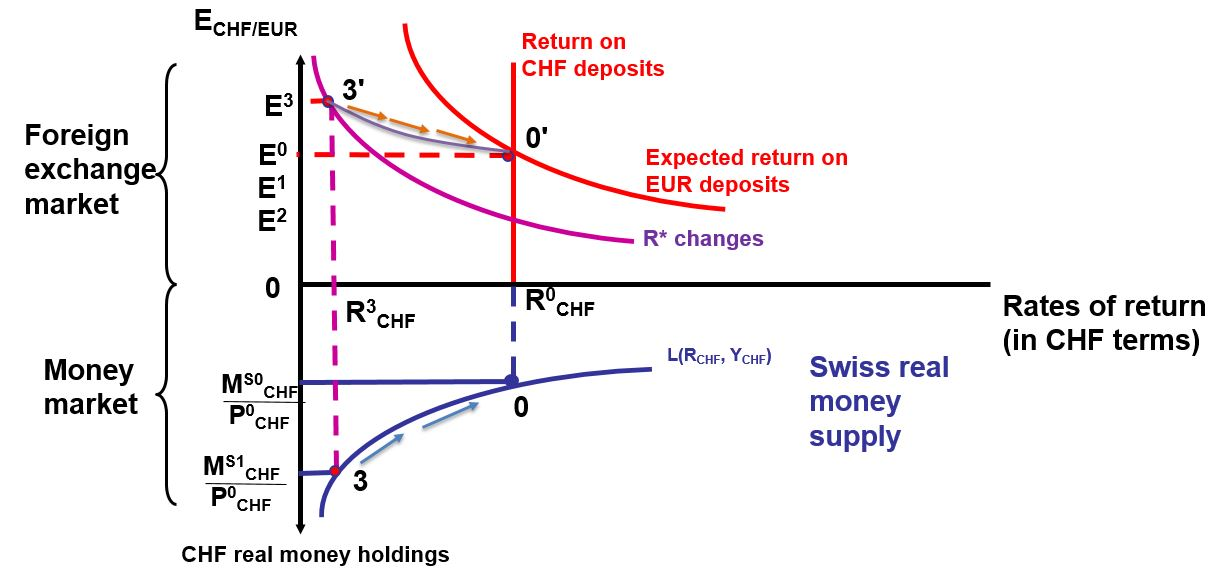
\includegraphics[scale=0.65]{5k.JPG} 
\caption{Question 2.k} 
\label{5k}
\end{figure}

\end{document}